
%(BEGIN_QUESTION)
% Copyright 2007, Tony R. Kuphaldt, released under the Creative Commons Attribution License (v 1.0)
% This means you may do almost anything with this work of mine, so long as you give me proper credit

Examine this process trend, showing the response of the process variable to a series of step changes in the controller output (placed in manual mode):

$$\includegraphics[width=15.5cm]{i01726x01.eps}$$

What kind of problem do you see evident in this trend?  Based on what you see here, do you think the process might benefit from a controller with aggressive P, I, or D action?  Explain why or why not for each action.

\vskip 20pt \vbox{\hrule \hbox{\strut \vrule{} {\bf Suggestions for Socratic discussion} \vrule} \hrule}

\begin{itemize}
\item{} One way to manage this problem is to use an {\it adaptive-gain} controller.  Explain what this means and why it may work.
\item{} A more direct way to rectify the problem is to alter the opening characteristic of the control valve.  Assuming the control valve has an inherently {\it linear} characteristic now, would you recommend changing the characteristic to {\it quick-opening} or to {\it equal-percentage}?
\item{} Based on what you see here, does the controller need to be configured for {\it direct} action or for {\it reverse} action?
\end{itemize}

\underbar{file i01726}
%(END_QUESTION)





%(BEGIN_ANSWER)

This is a self-regulating process with a variable gain.  The variation in gain means that no one set of PID settings will be adequate for robust, stable control across the measurement range.  You may be able to tune the controller for good response at one setpoint, but not for a wide range of setpoints.  This problem must be fixed before there will be any hope of tuning it well.

%(END_ANSWER)





%(BEGIN_NOTES)

Adaptive-gain controllers change their proportional setting according to the process variable, canceling the variable gain of the process.

\vskip 10pt

Assuming this control valve is air-to-open, a {\it quick-opening} control valve would be a better characteristic.  This would yield more aggressive control over the process at low openings (near the shut position) and less aggressive control over the process at high openings (near the wide-open position).

It should be noted that different valve characterization will work only for self-regulating processes, where valve position and PV are closely related.  On integrating processes, where valve position and PV are not so directly related, the valve's characterization will not accurately map to the process characterization except over a narrow load range.

%INDEX% Control, PID tuning: predicting PID requirements based on open-loop response

%(END_NOTES)


